
\documentclass[12pt]{article}
\pagestyle{empty}
\setlength{\parskip}{0in}
\setlength{\textwidth}{6.8in}
\setlength{\topmargin}{-.5in}
\setlength{\textheight}{9.3in}
\setlength{\parindent}{0in}
\setlength{\oddsidemargin}{-.7cm}
\setlength{\evensidemargin}{-.7cm}

\usepackage{amsmath}
\usepackage{amsthm}
\usepackage{amstext}

\usepackage{graphicx}

\begin{document}


{\bf MAT 105 Quiz 1.1-1.4 (ivory) Fall 2009} \hspace{.4in} {\large Name} \hrulefill

\hrulefill

 \emph{Relax.  You have done problems like these before.  Even if these problems look a bit different, just do what you can.  If you're not sure of something, please ask! You may use your calculator.  Please show all of your work and write down as many steps as you can.  Don't spend too much time on any one problem.  Please leave the following grading key blank for me to use.  Do well.  And remember, ask me if you're not sure about something.}

\begin{center}

\begin{tabular}
{|l|c|c|c|c|c|c|c|c|c|c|c|c|} \hline

 Problems & \hspace{5 pt} 1 \hspace{5 pt}  & \hspace{5 pt} 2 \hspace{5 pt} & \hspace{5 pt} 3 \hspace{5 pt} & \hspace{5 pt} 4 \hspace{5 pt} &  \hspace{5 pt} Total  \hspace{5 pt} & &  \hspace{5 pt} Grade \hspace{5 pt}  \\ \hline
&&&&& &&\\  
Points &&&&& &    \hspace{.8in}\% &  \\ 
&&&&& && \\  \hline
Out of & 16 & 16 & 6 & 12 &50 & & \\ \hline

\end {tabular}

\end{center}

\hrulefill

\begin{enumerate}

%%% Old 1.1-1.2, money/sales, everyday

\item The local burger joint by my house had a promotion this August.  Typically a double cheeseburger costs \$2.65.  Depending on the high temperature for the day, they would reduce the price of the double cheeseburger.  They reduced the price by \$0.01 for each degree in the temperature. For example, if the high temperature was 80 degrees Fahnrenheit, they would decrease the price by \$0.80, so the double cheeseburger would cost \$1.85.

\begin{enumerate}
\item Identify and name the variables in the story and state their units.
\vfill
\item Which variable is independent and which is dependent?
\vfill
\item Make a table showing the price of a cheeseburger when the temperature is 65 degrees, 75 degrees, and 90 degrees.
\vfill
\vfill
\vfill
\item Is the function increasing or decreasing?
\vfill
\end{enumerate}

\newpage

%%% Old 1.2-1.3, wedding, everyday
\item The table shows the cost for printing invitations for my friend's wedding last summer.  

\begin{center}
\begin{tabular} {|c|c|c|c|c|} \hline
$I$ & 10 & 50 & 125 & 200 \\ \hline
$C$ & 30 & 100 & 150 & 200 \\ \hline
\end{tabular}
\end{center}

In the table, $I$ = number of invitations ordered and $C$ = total printing cost  (\$).

\begin{enumerate}
\item What is the cost for ordering 50 invitations?

\emph{Don't forget the units.}
\vfill
\item Approximately what is the cost for ordering 150 invitations?
\vfill
\item Draw a graph illustrating this information.  \emph{Be sure your axes are labeled and evenly scaled.  Plot the points given and sketch in a smooth line or curve connecting them.}

\vfill
\begin{center}
\scalebox {.8} {
\includegraphics [width = 6in] {graphPaper.pdf}}
\end{center}
\vfill

\item Does your answer to part b agree with your graph?  (Yes or no)  If no, what would a better answer be?
\vfill
\end{enumerate}

\newpage

%%% Old 1.3, Minnesota, fun
\item The 2008 Minnesota State Fair was very well attended.  The graph below shows the daily attendance for each day of the fair.

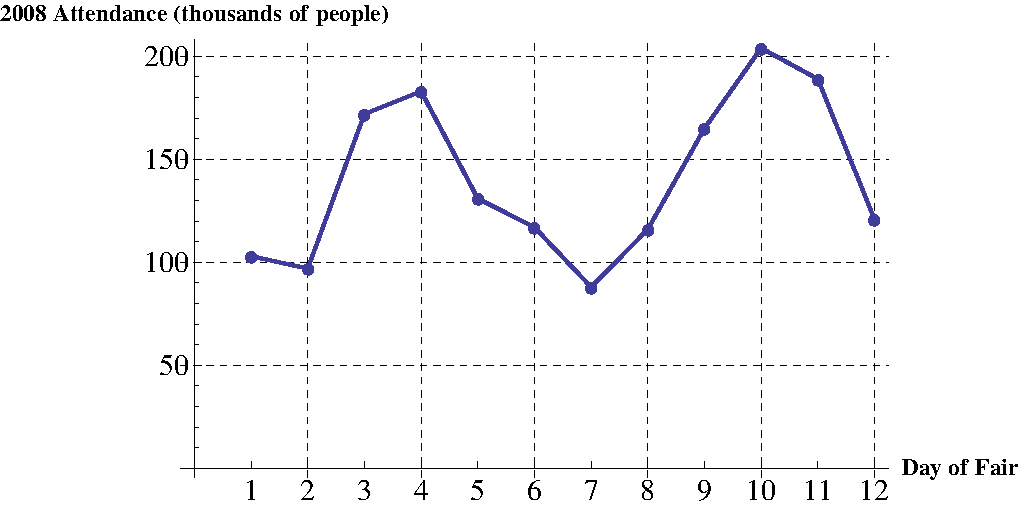
\includegraphics [width = 6in] {stateFair2008}

\begin{enumerate}
\item What was the approximate attendance for the second day of the fair?
\vfill
\item For how many days was the attendance greater than 150,000 people?
\vfill
\item In that year the State Fair began on a Thursday.  What do you think causes the attendance to peak for a given day?  Please write a sentence explaining your answer.
\vfill
\end{enumerate}
\newpage

%%% old 1.4, sports, fun
\item The Preakness Stakes is the second race in horse racing annual Triple Crown.  In the 2009 Preakness Stakes, the horse Rachel Alexrandra won with a time of 1 minute and 55.08 seconds.

\begin{enumerate}
\item Convert this time into decimal minutes.
\vfill
\vfill
\item The Preakness Stakes track is exactly 9.5 furlongs.  The furlong is an old measurement from medieval times.  Hence the horse's speed was 4.95 furlongs per minute, as you can check.  How fast is that speed in miles per hour?  \emph{Use 1 furlong = 660 feet and 1 mile = 5,280 feet.}
\vfill
\vfill
\vfill
\end{enumerate}

\end{enumerate}

\end{document}
